\chapter{Implementation}
Based on the methodology, this chapter presents the specific implementation carried out in this project, along with step-by-step instructions to run the demo and reproduce the results. The complete project repository, including all datasets and scripts, is available at \url{https://github.com/phmkhali/bias-detector-en-de}.

\section{Environment Setup and Project Structure}
    \subsection{System Environment and Hardware}
    The project was developed on macOS using Python 3.12.4. A virtual environment was used, and all dependencies were installed via the \texttt{requirements.txt} file using \texttt{pip3}. No manual installation steps were needed beyond this. During development, both GPU and CPU were used to test training and inference performance, with device selection handled dynamically. The final model for the demo and evaluation was trained on the CPU to ensure full compatibility and reproducibility without relying on a GPU. To ensure reproducibility, random seeds were fixed across all libraries and backends. The application is started via Streamlit. Further usage instructions are provided in \autoref{section:reproduction_guide}.

\subsection{Directory Layout}
    \autoref{fig:file_tree} shows the directory structure with the relevant files for the final implementation. The folder contains additional files related to the original datasets and scripts used for data conversion. These supplementary files are intended for comprehension and reproducibility purposes but are not required for the final model.

    \vspace{0.8em} 
    \begin{figure}[htb]
        \centering
        \scalebox{0.8}{\begin{forest}
  for tree={
    font=\ttfamily,
    grow'=0,
    child anchor=west,
    parent anchor=south,
    anchor=west,
    calign=first,
    edge path={
      \noexpand\path [draw, \forestoption{edge}]
      (!u.south west) +(7.5pt,0) |- (.child anchor) \forestoption{edge label};
    },
    before typesetting nodes={
      if n=1
        {insert before={[,phantom]}}
        {}
    },
    fit=band,
    before computing xy={l=15pt},
  }
[bias-detector-en-de
    [datasets
      [dataset.csv]
      [join\_datasets.py]
      [lardelli\_final.csv]
      [mgente\_final.csv]
      [tatoeba\_final.csv]
    ]
    [model\_output]
    [app.py]
    [fine-tuning.ipynb]
    [translate.py]
    [utils.py]
  ]
\end{forest}

}
        \caption[Relevant files of the final implementation]{Relevant files of the final implementation}
        \label{fig:file_tree}
    \end{figure}
    \vspace{0.8em} 


\section{Core Components and Data Flow}
    \subsection{Datasets Folder}
        The \texttt{datasets} folder contains the processed datasets used for training and evaluation of the bias detection model. It includes the final combined dataset \texttt{dataset.csv} as well as intermediate datasets derived from individual sources: \texttt{lardelli\_final}, \texttt{mgente\_final}, and \texttt{tatoeba\_final}. The \texttt{join\_datasets} script facilitates the concatenation of these datasets into a unified dataset. The script is designed to support iterative sampling by specifying sample sizes for biased and neutral classes with a fixed random seed. It merges the sampled subsets, shuffles the combined data, and performs data integrity checks. 

    \subsection{Fine-tuning Notebook and Model Output}
        The \texttt{fine-tuning.ipynb} notebook performs model initialization, training, evaluation, and testing. It loads the \texttt{mBERT} model and trains it on \texttt{dataset.csv}. Training artifacts are saved in the \texttt{model\_output} folder with checkpoints, configuration files, tokenizer files, and training metadata. The training process ran for six epochs due to early stopping and took approximately 18 minutes and 32 seconds on the development machine. 

    \subsection{Streamlit Application}
        The \texttt{app.py} file is the main entry point for the Streamlit interface.\footnote{Parts of the code were generated with AI and subsequently refined by the author; see Appendix \ref{appendix:ai_code} for details.}
        It loads the fine-tuned model and tokenizer from the \texttt{model\_output} directory and sets up the classification pipeline. In the automatic tab, users enter English text, which is translated using \texttt{translate.py}. In the manual tab, users enter both the original and translated sentences directly.\footnote{Screenshots of these tabs are shown in Figures~\ref{fig:demo_tab_1}, \ref{fig:demo_tab_2}, and \ref{fig:demo_multi_sentence}.} \texttt{translate.py} wraps the pre-trained OpusMT EN-DE model from Hugging Face. The main function, \texttt{translate\_batch}, takes a list of English sentences, tokenizes them, and uses the model's \texttt{generate} method to return a list of decoded German translations. The resulting sentence pairs from both tabs are passed to functions in \texttt{utils.py}. This module handles sentence splitting, optional translation, and model inference. It processes each sentence pair, predicts whether it contains gender bias, and formats the output with confidence scores for display in the interface.

        \vspace{0.8em}
        \begin{figure}[H]
            \centering
            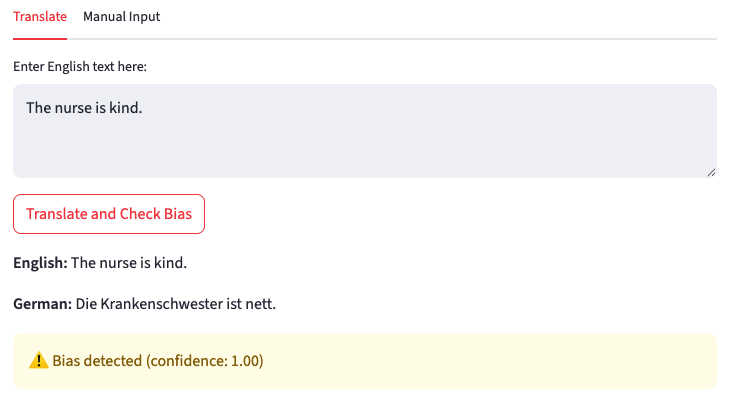
\includegraphics[width=0.75\textwidth]{demo_tab_1.png}
            \caption[Streamlit Demo: Automatic Translation Tab]{Streamlit Demo: Automatic Translation Tab showing correct identification of bias in stereotypical occupational gender assignment}
            \label{fig:demo_tab_1}
        \end{figure}
        \vspace{0.8em}

        \begin{figure}[H]
            \centering
            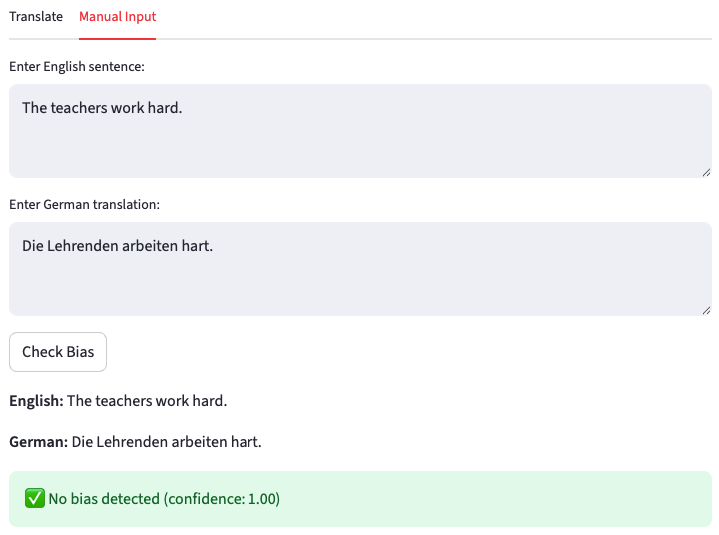
\includegraphics[width=0.75\textwidth]{demo_tab_2.png}
            \caption[Streamlit Demo: Manual Translation Tab]{Streamlit Demo: Manual Translation Tab showing no bias detected due to use of GFL}
            \label{fig:demo_tab_2}
        \end{figure}
        \vspace{0.8em}

        \begin{figure}[H]
            \centering
            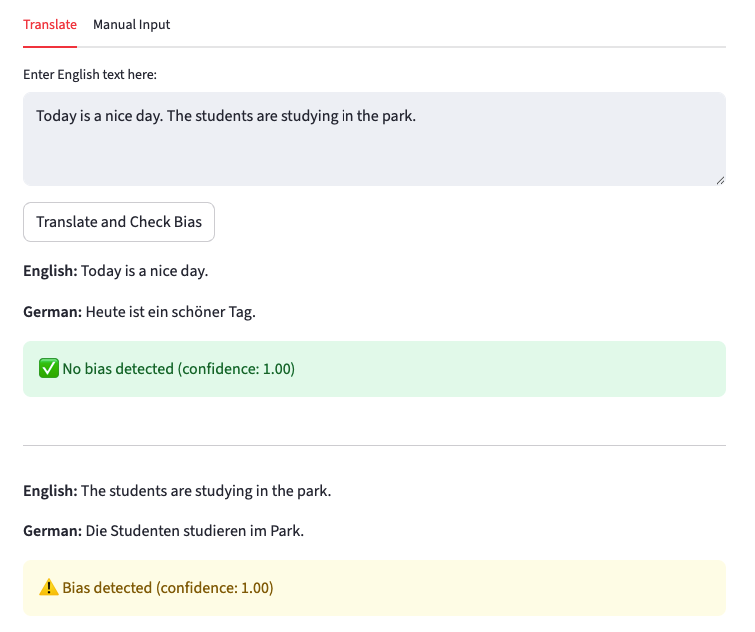
\includegraphics[width=0.8\textwidth]{demo_multi_sentence.png}
            \caption[Streamlit Demo: Multi Sentence Translation]{Streamlit Demo correctly splitting and labeling two sentences as neutral and biased}
            \label{fig:demo_multi_sentence}
        \end{figure}
        \vspace{0.8em}

\section{Reproduction Guide} \label{section:reproduction_guide}
   The setup process for the Streamlit demo app includes creating a Python virtual environment, installing required packages, and running the application. This guide covers these steps for macOS/Linux and Windows. \textbf{Note:} The pre-trained model is not included in the GitHub repository due to size restrictions. It can be downloaded separately via the provided Google Drive link.\footnote{ \href{https://drive.google.com/drive/folders/11WMb0od_U_sQsUGD0t4DjQwcefI3r_kK?usp=sharing}{Google Drive link} for the model.} If the pre-trained model is not present, the \texttt{fine-tuning.ipynb} notebook must be executed first to train and save the model before launching the demo.
\paragraph{Installation Steps}

\begin{enumerate}
    \item Open a terminal (macOS/Linux) or PowerShell (Windows).
    
    \item Clone the GitHub repository and download the pre-trained model:
        
    \begin{tcolorbox}[colback=gray!10, colframe=gray!50, breakable, boxrule=0.4pt, sharp corners]
\begin{verbatim}
git clone https://github.com/phmkhali/bias-detector-en-de
cd bias-detector-en-de
\end{verbatim}
    \end{tcolorbox}
    
    \textit{Download the model}
    
    \begin{tcolorbox}[colback=gray!10, colframe=gray!50, breakable, boxrule=0.4pt, sharp corners]
\begin{verbatim}
# Manually download from the provided Google Drive link above
# and place the model_output folder into the directory
\end{verbatim}
    \end{tcolorbox}
    
    \item Create and activate a Python virtual environment:
    
    \textit{macOS / Linux}
    
    \begin{tcolorbox}[colback=gray!10, colframe=gray!50, breakable, boxrule=0.4pt, sharp corners]
\begin{verbatim}
python3 -m venv venv
source venv/bin/activate
\end{verbatim}
    \end{tcolorbox}
    
    \textit{Windows}
    
    \begin{tcolorbox}[colback=gray!10, colframe=gray!50, breakable, boxrule=0.4pt, sharp corners]
\begin{verbatim}
python -m venv venv
.\venv\Scripts\activate
\end{verbatim}
    \end{tcolorbox}
    
    \item Install the required packages:
    
    \textit{macOS / Linux}
    
    \begin{tcolorbox}[colback=gray!10, colframe=gray!50, breakable, boxrule=0.4pt, sharp corners]
\begin{verbatim}
pip3 install -r requirements.txt
\end{verbatim}
    \end{tcolorbox}
    
    \textit{Windows}
    
    \begin{tcolorbox}[colback=gray!10, colframe=gray!50, breakable, boxrule=0.4pt, sharp corners]
\begin{verbatim}
pip install -r requirements.txt
\end{verbatim}
    \end{tcolorbox}
    
    \item (Only necessary if the \texttt{model\_output} directory was not downloaded and added to the repository) Run the \texttt{fine-tuning.ipynb} notebook manually to generate the model.

    \item Run the Streamlit app:
    
    \textit{macOS / Linux}
    
    \begin{tcolorbox}[colback=gray!10, colframe=gray!50, breakable, boxrule=0.4pt, sharp corners]
\begin{verbatim}
python3 -m streamlit run app.py
\end{verbatim}
    \end{tcolorbox}
    
    \textit{Windows}
    
    \begin{tcolorbox}[colback=gray!10, colframe=gray!50, breakable, boxrule=0.4pt, sharp corners]
\begin{verbatim}
streamlit run app.py
\end{verbatim}
    \end{tcolorbox}
\end{enumerate}
